%% USPSC-Cap2-Desenvolvimento.tex 


\chapter[Metodologia]{Metodologia}

    \section{Fundamentos}
    
        \subsection{Tratamento de Dados}
            Em relação às etapas de tratamento de dados necessárias em um projeto de aprendizagem de máquina, vamos nos deter a dois pontos principais: outliers e dados faltantes.\newline 
        
            \textbf{Dados espúrios}\par
            Um outlier "é uma observação que se encontra a uma distância anormal de outros valores em uma amostra aleatória de uma população. (...) Outliers podem distorcer a distribuição sumária de valores de atributos em estatísticas descritivas como média e desvio padrão e em gráficos como histogramas e gráficos de dispersão, comprimindo o corpo dos dados." \cite{portal2018}\newline
        
            \textbf{Dados faltantes}\par
            Durante o desenvolvimento de um modelo, "é comum existirem, dentre as variáveis preditivas, algumas que possuem dados não preenchidos (missings), sendo necessário assim adotar algum procedimento para tratamento destas variáveis." \cite{assuncao2012}\newline

	    \subsection{Bliblioteca Scikit-learn}
	    O scikit-learn "é uma biblioteca da linguagem Python desenvolvida especificamente para aplicação prática de machine learning. Esta biblioteca dispõe de ferramentas simples e eficientes para análise preditiva de dados, é reutilizável em diferentes situações, possui código aberto, sendo acessível a todos e foi construída sobre os pacotes NumPy, SciPy e matplotilib". \cite{didatica2020}

        \subsection{Algoritmos de regressão}
	    De acordo com a Oper Data \cite{oper2020}, os problemas de Machine Learning "são divididos em três subáreas principais: classificação, regressão e clustering.". Para esse trabalho, serão de especial interesse os algoritmos de regressão, dentre os quais destacam-se os seguintes grupos:\par

		    \textbf{Árvores de decisão}\par
		    A árvore de decisão "está entre os métodos mais comuns aplicados ao aprendizado de máquina. Tais algoritmos subdividem progressivamente os dados em conjuntos cada vez menores e mais específicos, em termos de seus atributos, até atingirem um tamanho simplificado o bastante para ser rotulado. Para isso é necessário treinar o modelo com dados previamente rotulados, de modo a aplicá-lo a dados novos." \cite{digitalhouse2021}\newline

		    \textbf{Regressão logística}\par
		    A regressão logística "é uma técnica estatística que tem como objetivo produzir, a partir de um conjunto de observações, um modelo que permita a predição de valores tomados por uma variável categórica, frequentemente binária, em função de uma ou mais variáveis." \cite{gonzalez2018}\newline
		    
		    \textbf{Support vector machines}\par
		     Algoritmos de máquina de vetores de suporte (em inglês, Support Vector Machines, ou SVM) "têm como objetivo a determinação de limites de decisão que produzam uma separação ótima entre classes por meio da minimização dos erros." \cite{nascimento2009}\newline
		    
		    \textbf{Random forest}\par
		    O algoritmo de Random Forest leva esse nome por "criar muitas árvores de decisão, de maneira aleatória, formando o que podemos enxergar como uma floresta, onde cada árvore será utilizada na escolha do resultado final". \cite{didatica2019}\newline
		    
		    
		    \textbf{Redes neurais}\par
		    Redes Neurais "são um formato de estrutura de dados inspirada nas redes de neurônios do cérebro humano (...) organizadas em uma lógica de camadas e nós dentro dos códigos de programação, sugerindo uma estrutura vagamente similar ao que ocorre com os neurônios".\cite{ilumeo2020}\newline
		    
	    \subsection{Avaliação de algoritmos de regressão}
	    Para comparar e selecionar modelos de aprendizagem de máquina, é necessário definir métricas que possam ser utilizadas como critério de avaliação. Entre elas, podemos destacar três:\newline
	
	        \textbf{R Square (Quadrado de R)}\par
	        A métrica R Square "mede quanta variabilidade na variável dependente pode ser explicada pelo modelo. É o quadrado do Coeficiente de Correlação (R), e por isso é chamada de R Square". \cite{towards2020} (tradução do autor).\newline
	
        	\textbf{Erro médio quadrático}\par
	        Em oposição à medida R Square, que é "uma medida relativa de quão bem o modelo se ajusta a variáveis dependentes", o Erro Médio Quadrático "é uma medida absoluta da qualidade do ajuste", e pode ser calculado pela soma do quadrado do erro de predição, que é o valor real de uma observação menos o valor previsto, e depois dividido pelo número de observações." \cite{towards2020} (tradução do autor)\newline
	
	        \textbf{Erro Médio Absoluto}\par
	        O Erro Médio Absoluto "é similar ao Erro Médio Quadrático. No entanto, em vez da soma do quadrado do erro no EMQ, EMA utiliza a soma do valor absoluto do erro." \cite{towards2020} (tradução do autor)

    \section{Trabalhos relacionados}
    
        \textbf{Popularidade de filmes}\par

        Entre os trabalhos já realizados sobre a aplicação de algoritmos de aprendizagem de máquina na predição de popularidade de filmes, podemos destacar o artigo "Prediction of Movies popularity Using Machine Learning Techniques" ("Previsão da popularidade de filmes usando técnicas de aprendizado de máquina", tradução do autor).\par
        A metodologia utilizada pelo autor é descrita da seguinte forma: "criamos um conjunto de dados e, em seguida, o transformamos e aplicamos abordagens de aprendizado de máquina para construir modelos eficientes que podem prever a popularidade dos filmes." \cite{afzal2016} (tradução do autor)\par
        Entre os resultados obtidos, o autor destaca: "Depois de fazer a classificação, descobrimos que nossos melhores resultados são alcançados por meio de regressão logística. Os atributos que mais contribuíram para a informação são o metascore e o número de votos de cada filme, os Oscars conquistados pelos filmes e a quantidade de telas que o filme vai passar." \cite{afzal2016}\newline

        \textbf{Predição de bilheteria}\par
        Em relação à predição de bilheteria para um filme, Quader et al destacam a importância dos metadados no artigo "Performance evaluation of seven machine learning classification techniques for movie box office success prediction" ("Avaliação de desempenho de sete técnicas de classificação de aprendizado de máquina para previsão de sucesso de bilheteria de filmes", tradução nossa). Os autores buscam "realizar uma comparação de desempenho entre vários métodos de aprendizado de máquina. Escolhemos sete técnicas de aprendizado de máquina para esta comparação, como Support Vector Machine (SVM), Regressão Logística, Multilayer Perceptron Neural Network, Gaussian Naive Bayes, Random Forest, AdaBoost e Stochastic Gradient Descent (SGD). Todos esses métodos prevêem um valor aproximado de lucro líquido de um filme, analisando dados históricos de diferentes fontes como IMDb, Rotten Tomatoes, Box Office Mojo e Meta Critic." \cite{quader2017} (tradução do autor)\par
        Entre as conclusões, os autores citam elementos que podem facilitar ou dificultar a análise: "Se a condição econômica e política de um país não é estável, não importa o quão bem o filme seja feito, não haverá ninguém para assisti-lo. Portanto, incluir o PIB de um país como um atributo é uma boa opção para uma análise posterior. Também sugerimos analisar e incluir o número de público para análise. Podemos obter o número de audiência anual usando o total de ingressos vendidos em um determinado ano. Incluir esses atributos tornará a previsão mais precisa."
    
    \section[Desenvolvimento]{Desenvolvimento}

        \subsection{Considerações iniciais}
        Este capítulo descreve as etapas de desenvolvimento dos modelos de previsão de chances de indicação e premiação no Oscar, detalhando as escolhas realizadas e os procedimentos adotados no processo. São explicados também os resultados atingidos, os problemas enfrentados e as melhorias que podem ser realizadas em trabalhos futuros.
    
        \subsection{Atividades realizadas}
    
            \textbf{Obtenção dos dados}\par

            Foi escolhida como fonte de dados para o trabalho a database "The Movies Dataset", da plataforma Kaggle. Trata-se de um conjunto incluindo "metadados para todos os 45.000 filmes listados no conjunto de dados Full MovieLens. O conjunto de dados consiste em filmes lançados em ou antes de julho de 2017. Os dados incluem elenco, equipe, palavras-chave do enredo, orçamento, receita, pôsteres, datas de lançamento, idiomas, empresas de produção, países, contagens de votos TMDB e média de votos".\cite{kaggle2017}\par
            
            A base de dados ``The Oscar Award, 1927 - 2020'' foi utilizada para complementar os metadados, adicionando a eles as informações de indicações e vitórias na premiação.\cite{kaggle2019}\newline

            \textbf{Limpeza e tratamento dos dados}\par
            
            O primeiro desafio relacionado à limpeza e tratamento dos dados aparece na base \citeonline{kaggle2019}. Embora a base esteja bastante completa em todas os outras colunas, a coluna 'film' - justamente a que traz o nome do filme relacionado àquela premiação - está nula em 304 linhas.
            
            \begin{figure}[htb]
            	\caption{\label{faltantes_film}Dados faltantes na coluna film}
            	\begin{center}
            		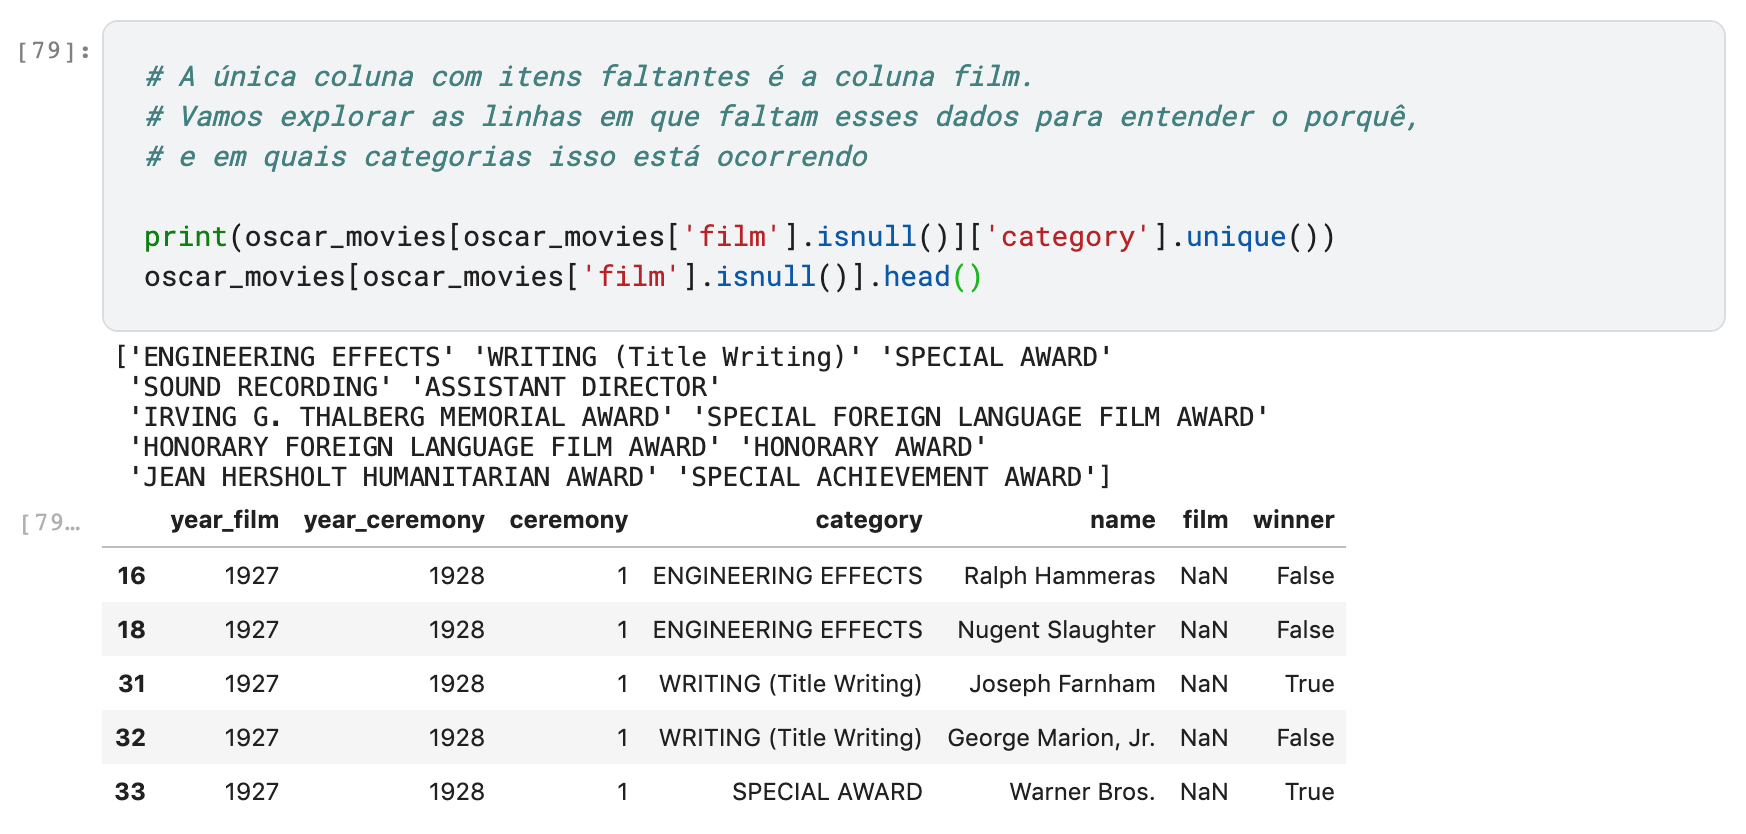
\includegraphics[scale=0.5]{faltantes_film.png}
            	\end{center}
            	\legend{Fonte: trabalho nosso}
            \end{figure}
            
            Em algumas dessas categorias, nota-se que se trata de prêmios honorários, humanitários ou de conjunto da obra. Esses dados foram desconsiderados, já que não se referem a um filme específico.
            
            Já para duas das categorias que apresentam dados faltantes - "SPECIAL FOREIGN LANGUAGE FILM AWARD"
            e "HONORARY FOREIGN LANGUAGE FILM AWARD" -, é possível perceber que o nome se encontra na coluna 'name', precisando apenas de tratamento em alguns casos, podendo então ser transferido para a coluna "film".
            
            Outras linhas com dados faltantes na coluna 'film' são de obtenção difícil ou imprecisa: um assistente de direção, por exemplo, pode ter tido mais de um filme lançado num mesmo ano, o que faria a checagem dos dados restantes muito trabalhosa. Essas colunas serão ignoradas, nos deixando ao final com 10098 linhas completas no dataset.
            
            Um fato que pode ser observado analisando-se esses dados restantes é que algumas das categorias tiveram mudanças de nomes - como foi o caso na premiação de filme de língua estrangeira. Já outras categorias desapareceram da premiação ("melhor filme em preto e branco") ou foram incluídas. A categoria mais recente incluída na premiação é a de melhor filme de animação, criada em 2002. \cite{usatoday2002}.
            
            Por esse fator, iremos desconsiderar filmes anteriores a essa data. Essa abordagem tem ainda a vantade de delimitar um recorte cronológico mais coeso, permitindo a visualisação de tendências, o que seria improvável na análise total de quase 100 anos de premiação. Iremos desconsiderar ainda a premiação de edição de som (sound editing), que foi descontinuada em 2019, a única removida após o ano de 2002.\cite{deadline2020}
            
            Algumas dessas categorias também precisaram de consolidação, já que seus nomes apareciam de formas diferentes. Foram utilizados os nomes mais recentes.
            
            O passo seguinte é integrar os esquemas dos dois datasets. Para isso, vamos considerar que um filme é o mesmo nos dois datasets caso seu nome e ano apresentem correspondência. Para a análise de nome, serão observadas as colunas 'title' (em alguns casos, também a 'original\_title') do dataset de metadados, e a coluna 'film' do dataset do Oscar.

            Para análise dos anos, foi criada no dataset de metadados uma coluna 'release\_year', extraindo o ano da coluna 'release\_date'. Esse valor será comparado com a coluna 'year\_film' do dataset do Oscar.

            Mas para fazer essa união entre as duas tabelas, foi também necessário normalizar nomes nas duas tabelas, adicionando-se as colunas "normalized\_title" e "normalized\_original\_title". Alguns dos desafios encontrados nesse estágio foram:

            \begin{itemize}
                \item remoção de caracteres especiais e capitalização;
                \item existência, na tabela do Oscar, de filmes com título em inglês ou no original em outra língua;
                \item títulos estilizados (geralmente com pontuação no nome);
                \item filmes com anos diferentes nos dois datasets.
            \end{itemize}

            Esse último item diz respeito à observação de filmes com ano de lançamento ('release\_year') diferentes do ano na tabela do Oscar (coluna 'year\_film'). Um exemplo é o filme 'Y tu mamá también', cuja coluna 'year\_film' tem valor 2002 no dataset do Oscar e 2001 no dataset de metadados. Nesses casos, a coluna 'year\_film' será corrigida para o valor presente na tabela de metadados.


            Com essas informações, já é possível relacionar entre as tabelas 759 dos 942 filmes existentes no dataset do Oscar. Para os restantes 183 filmes, dois desafios especiais se deram:\par

            \begin{itemize}
                \item títulos em inglês diferentes de acordo com o país - por exemplo, o filme "Harry Potter e a Pedra Filosofal", lançado nos Estados Unidos e Índia como "Harry Potter and the Sorcerer's Stone" e nos outros países de língua inglesa "Harry Potter and the Philosopher's Stone"; \cite{yahoo2000};\par
                \item títulos divergentes entre as duas tabelas (como "Mt. Head" na tabela do Oscar, que consta como "Mount head" na tabela de metadados de filmes).\par
            \end{itemize}

            Para esses casos, foi realizada uma análise de similaridade entre os títulos não encontrados nas duas tabelas, utilizando a biblioteca nativa difflib do Python, e uma análise caso a caso.
            
            Nessa análise, foram considerados como o mesmo filme:\newline
            
            
            
            
            
            
            
            
            Para adicionar as informações dos Oscars ao The Movies Dataset, vamos criar colunas no formato one-hot encoding para inserir as informações de nomeação e vitória em cada categoria para cada filme.\newline
            
            
            
            
            \textbf{Arcabouço de análise exploratória}\par
            Após unificados os dados, será realizada análise exploratória com Pandas, Numpy, e Scikit Learn para conferir a natureza dos dados, a existência de dados faltantes ou inconsistentes e a existência de tendências que auxiliem na construção dos modelos.\newline
    
            \textbf{Criação de modelos}\par
            Serão criados modelos de regressão para inferir a chance de premiação utilizando diferentes algoritmos, entre os quais árvores de decisão, regressão logística, support vector machines, random forest e redes neurais.\newline
    
            \textbf{Avaliação comparativa dos resultados}\par
            Avaliação comparativa dos resultados usando as métricas de mean squared error, root mean squared error, e mean absolute error.\newline
    
            \textbf{Avaliação de importância dos metadados}\par
            Avaliação da importância de cada fator (metadado) na previsão, baseando-se no feedback dos algoritmos testados.\newline
    
            \textbf{Interpretação dos resultados}\par
            Interpretação dos resultados para elaboração das conclusões com indicação das técnicas mais promissoras.\newline

        \subsection{Resultados obtidos}

% cola para inserir figura
% \newpage
% \begin{figure}[htb]
% 	\caption{\label{fig_EstruturaTrabAcad}Estrutura do trabalho acadêmico}
% 	\begin{center}
% 		\includegraphics[scale=0.5]{USPSC-EstruturaTrabAcad.jpg}
% 	\end{center}
% 	\legend{Fonte: \citeonline{nbr14724}}
% \end{figure}
